\subsection{Discrete Controller Verification}\label{ssec:discreteControllerVerification}
It is necessary to verify that the discretized controller matches the original continuous one, and is also able to maintain the Cubli in the upright position. This is done firstly, by simulating the feedback system and comparing the newly made discrete controller with the continuous simulation from \figref{PositionResponse}, see \figref{fig:discreteVsContinuousSimulation}.
%
\begin{minipage}{\linewidth}
  \begin{minipage}{0.45\linewidth}
    \begin{figure}[H]
      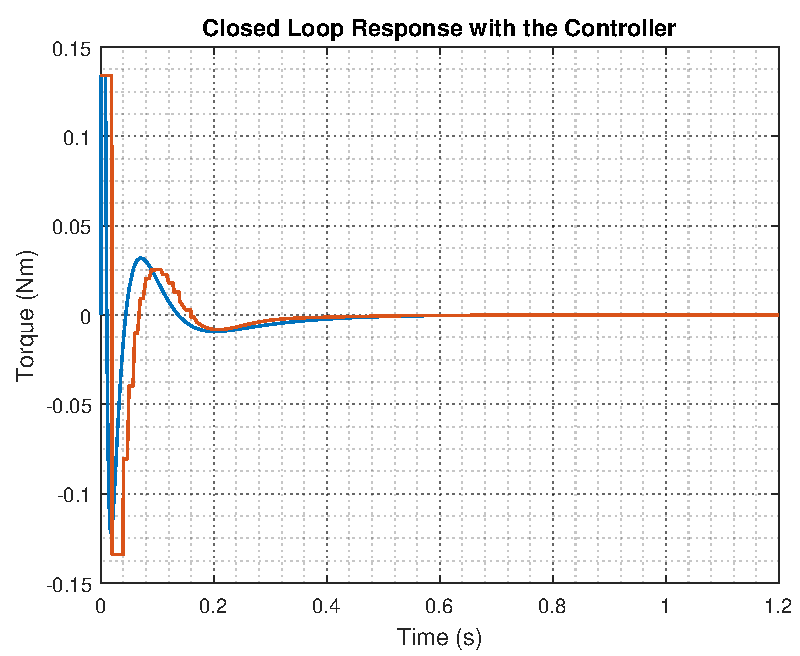
\includegraphics[scale=.53]{figures/torqueComp.pdf}
      \centering
      \vspace{-.4cm}
      \captionsetup{justification=centering}
      \captionof{figure}{Controller's output (torque) response in the control loop with the continuous (blue) and discrete (red) controllers}
      \label{fig:discreteVsContinuousOutputController}
    \end{figure}\vspace{-5mm}
  \end{minipage}
  \hspace{0.03\linewidth}
  \begin{minipage}{0.45\linewidth}
    \begin{figure}[H]
      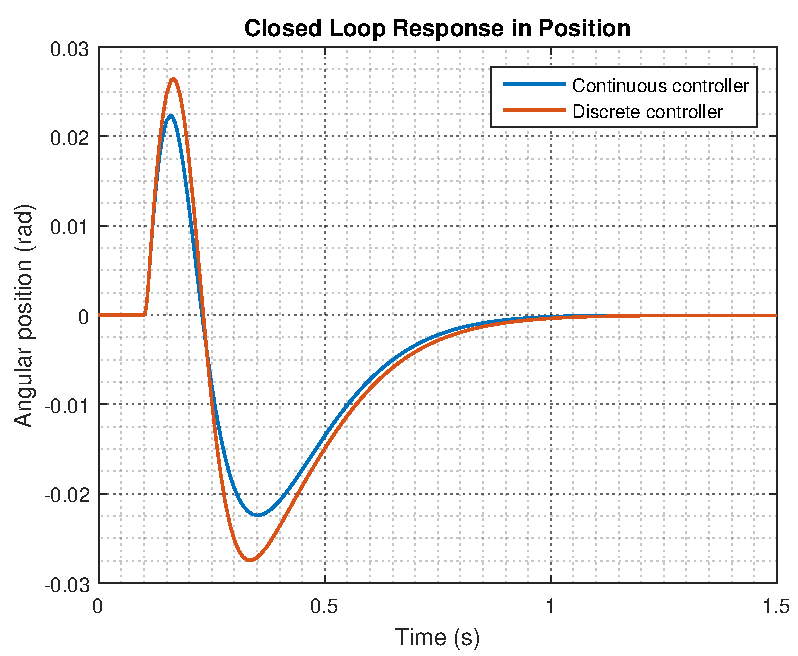
\includegraphics[scale=.53]{figures/positionComp.pdf}
      \centering
      \vspace{-.4cm}
      \captionsetup{justification=centering}
      \captionof{figure}{Closed loop response of the continuous (blue) and discrete (red) controllers}
      \label{fig:discreteVsContinuousSimulation}
    \end{figure}\vspace{-5mm}
  \end{minipage}
\end{minipage}

In \figref{discreteVsContinuousSimulation}, the system is given an initial condition of. The discretized controller seems to fulfill the basic requirement of putting back the Cubli in the upright (\si{0^{\circ}}) position. However, ...